\chapter{Study Area and Data}
\label{ch:data}
\section{Study Site}
The study site (11.25--11.55$^\circ$\,E, 47.15--47.35$^\circ$\,N; approximately $23\times22$\,km$^2$) is centred on the city of Innsbruck in Tyrol, Austria (Fig.~\ref{fig:site}). The east--west oriented Inn valley, with a floor at about 580\,m above sea level, separates the steep south face of the Nordkette (up to 2300\,m) in the north from the Patscherkofel and the Stubai pre-Alps in the south; the Sill gorge (Wipptal) enters the valley from the south. Elevations within the site range from 552\,m to 2789\,m. The site therefore contains all regimes of geometric distortion and a strong land-cover contrast between the urbanised valley floor, extensive forests, alpine grassland and bare rock.

\begin{figure}[htbp]
\centering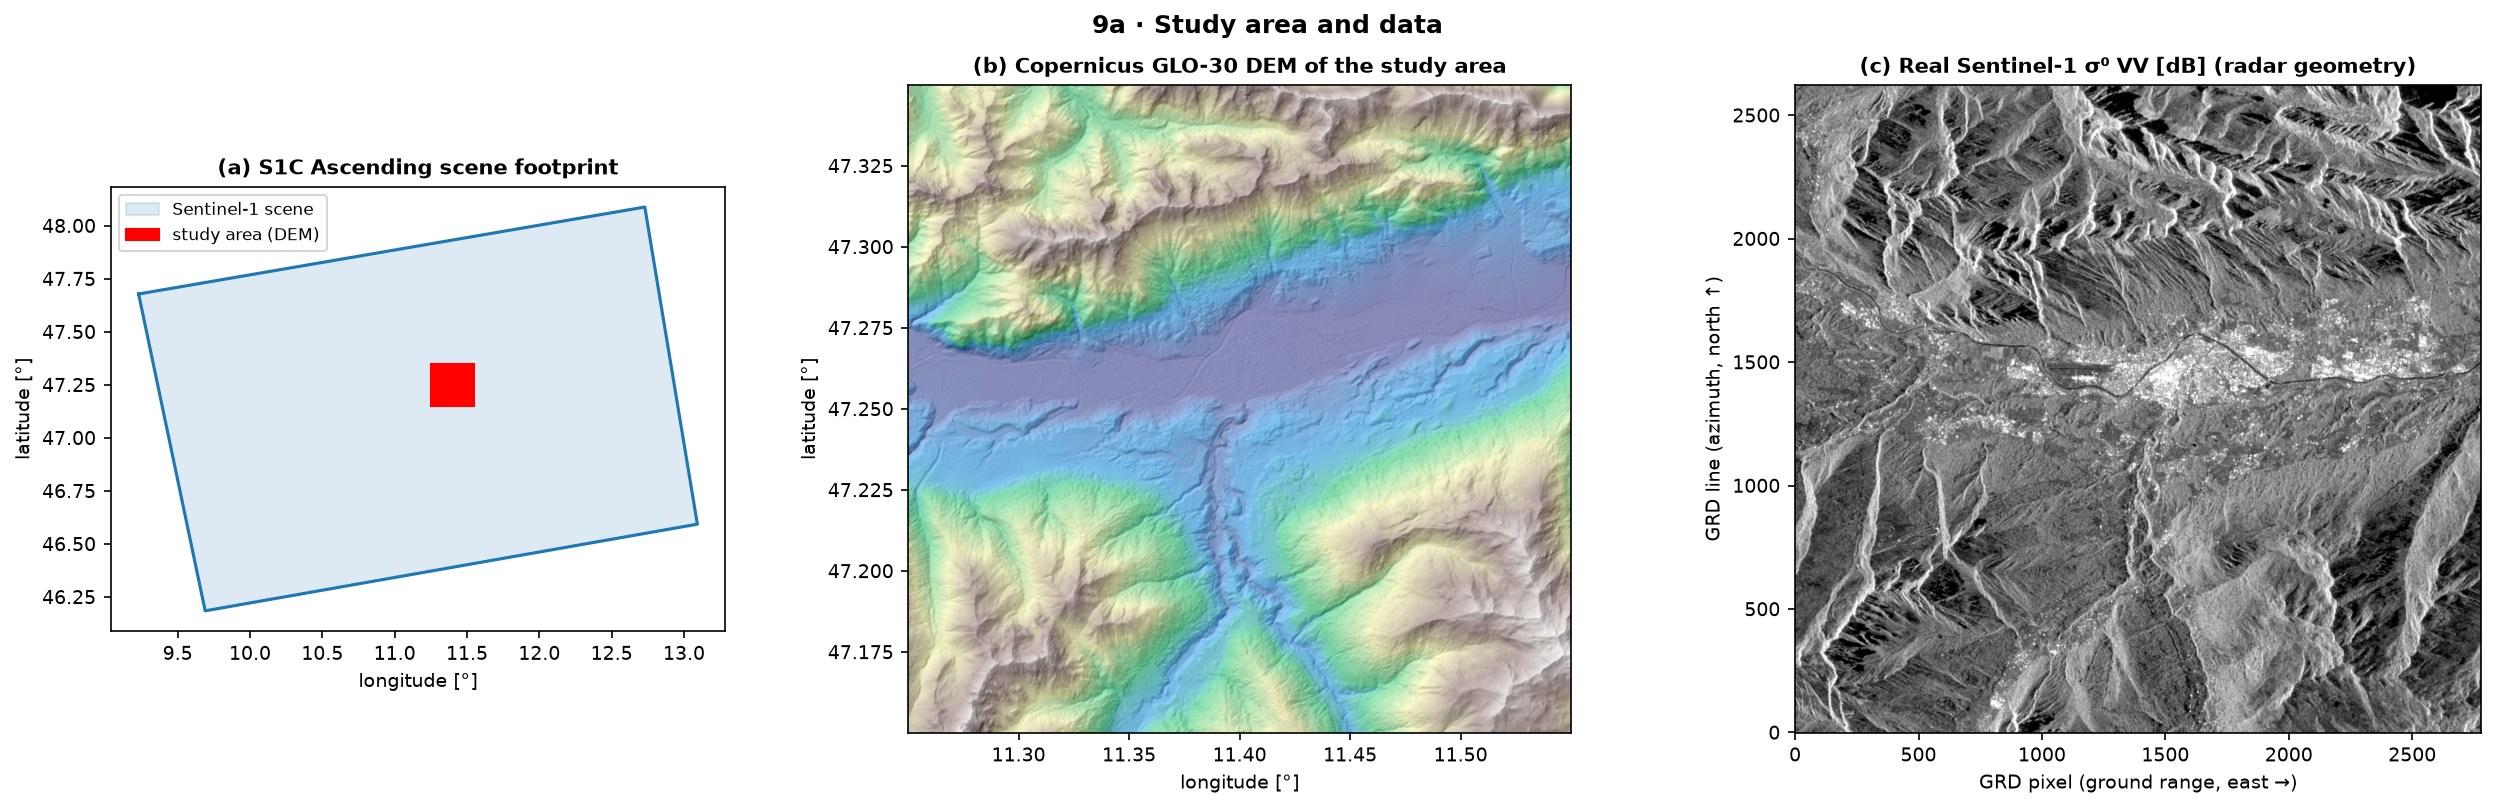
\includegraphics[width=\textwidth]{09a_study_area_data.png}
\caption[Study site and data]{Study site and data. (\textbf{a}) Footprint of the ascending Sentinel-1 scene and the study site (red). (\textbf{b}) Copernicus GLO-30 DEM of the study site. (\textbf{c}) Calibrated Sentinel-1 $\sigz$ (VV) of the study site in radar geometry.}
\label{fig:site}
\end{figure}

\section{Digital Elevation Model}
The Copernicus GLO-30 DEM~\cite{copdem} tile N47\,E011 was cropped to the study site, yielding $720\times1080$ samples at 1\,arcsec spacing (about 31\,m north--south and 21\,m east--west). GLO-30 heights refer to the EGM2008 geoid~\cite{pavlis2012}; they were converted to WGS84 ellipsoidal heights with the geoid undulation $N=\geoidN$\,m obtained from the EGM2008 model, as required by the orbit-based geocoding.

\section{Sentinel-1 Data}
Two Sentinel-1C Interferometric Wide-swath (IW) GRD high-resolution products in VV polarisation, one from an ascending and one from a descending pass, were selected as the most recent scenes in August--September 2025 that fully cover the site (Table~\ref{tab:s1}). The ascending pass looks east and the descending pass looks west, so that the two geometries illuminate opposite slopes. Only the window of each GRD image that covers the DEM (about $2600\times2780$ pixels of $10\times10$\,m) was read from the cloud-optimised file. For each product, the annotation provides the orbit state vectors (10\,s spacing), the zero-Doppler time of the first line and the azimuth time interval, 28 time-tagged SRGR polynomials, the geolocation grid (210 tie points) and the radiometric calibration look-up table~\cite{s1pd}.

\begin{table}[htbp]
\caption[Sentinel-1 data used in this study]{Sentinel-1 data used in this study. Incidence angle at mid-swath; window size in GRD pixels.}
\label{tab:s1}
\centering\small
\begin{tabularx}{\textwidth}{lXX}
\toprule
 & \textbf{Ascending} & \textbf{Descending}\\\midrule
Platform, mode, polarisation & \platAsc, IW GRDH, VV & \platDesc, IW GRDH, VV\\
Acquisition start (UTC) & \dateAsc, 17:06:22 & \dateDesc, 05:17:54\\
Absolute orbit & 4313 & 4291\\
Look direction & east & west\\
Incidence angle (mid-swath) & \incAsc$^\circ$ & \incDesc$^\circ$\\
Pixel spacing (range $\times$ azimuth) & $10\times10$\,m & $10\times10$\,m\\
Window covering the DEM & $2622\times2780$ & $2600\times2772$\\
\bottomrule
\end{tabularx}
\end{table}

\section{Land Cover}
The ESA WorldCover 2021 map at 10\,m resolution~\cite{worldcover} was sampled at the DEM grid by nearest-neighbour interpolation. Within the analysed area, tree cover represents 55\,\% of the pixels, grassland 26\,\%, built-up areas 7\,\%, bare or sparsely vegetated land 6\,\% and cropland 4\,\%; water, snow and ice, and moss and lichen together represent about 2\,\%. All data sets were accessed through the Microsoft Planetary Computer~\cite{planetary}.
